\begin{figure}[h]
    \centering
    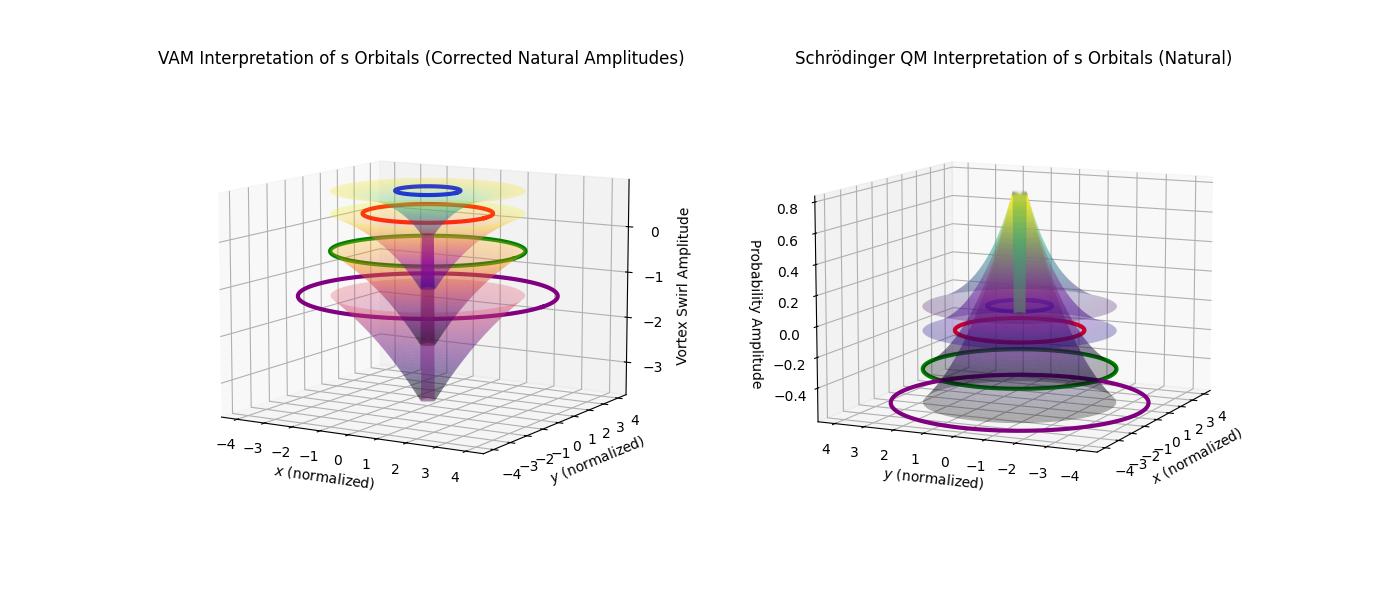
\includegraphics[width=0.7\textwidth]{vortex_diagram}
    \caption{Illustration of a vortex filament in \AE ther.}
    \label{fig:vortex}
\end{figure}

\subsection{The \AE ther is characterized by three fundamental constants:}\label{subsec:the-ae-ther-is-characterized-by-three-fundamental-constants:}

The Vortex \AE ther Model (VAM) posits a structured, vorticity-driven \AE ther as the fundamental medium governing physical interactions.
This model challenges the conventional relativistic framework by proposing an alternative description of time, mass, and energy



\begin{itemize}
    \item The vortex tangential velocity constant, given by: \[C_e = 1093845.63 \, \mathrm{m/s}\]
    \item The maximum coulomb force in the \AE ther, given by:\[F_{\text{Cmax}} = 29.053507 \, \mathrm{N}\]
    \item The Coulomb barrier (Vortex Core Radius), given by: \[r_c = 1.40897017 10^-15 m\]
\end{itemize}

These constants govern the dynamic behavior of the \AE ther, regulating vortex circulation velocity and providing upper limits for interactions within the \AE theric medium.
Unlike the archaic notion of a luminiferous medium, this \AE ther is envisioned as a non-viscous superfluid supporting vortex structures, enabling vorticity-driven interactions.
This perspective implies that mechanical information may be exchanged within the \AE ther at rates exceeding the traditional speed of light, challenging the relativistic limitations on causality.


\subsubsection*{Vorticity Flow and Stability}

\begin{itemize}
    \item The central aperture of a trefoil knot aligns along the z-axis, facilitating directed motion in this direction.
    \item The surrounding flat fluid retains a constant vorticity, maintaining directional stability.
\end{itemize}
Vorticity remains proportional to twice the angular velocity of the rotating core, stabilizing vortex propagation dynamics.


\subsection{Gravity as a Vorticity-Induced Pressure Gradient}\label{sec:gravity-as-a-vorticity-induced-pressure-gradient}
    \subsubsection{Electromagnetism as a Vortex Filament Network}\label{sec:electromagnetism-as-a-vortex-filament-network}
    \subsubsection{Experimental Predictions and Feasibility}\label{sec:experimental-predictions-and-feasibility}
    \subsubsection{Conclusion}\label{sec:conclusion}
    We have outlined a vortex-based approach to gravity and electromagnetism, As shown in Eq. \eqref{eq:vorticity}, the vorticity transport equation governs  The Vortex \AE ther Model offers a new perspective on fundamental forces,
    replacing spacetime curvature with fluid dynamics in an inviscid \AE ther.
    This framework provides a coherent mathematical model with experimentally testable predictions.
    While VAM provides an alternative to spacetime curvature, further work is needed to derive cosmological implications.
    How does VAM handle large-scale structure formation?
    Can it explain galactic rotation curves without dark matter?
    Future research will explore these avenues.









        \subsubsection{Derivation of the Density of the \AE ther ($\rho_\text{\AE}$)}\label{sec:derivation-of-the-density-of-the-ae{}ther-($rho_text{ae}$)}

        The energy density of a vorticity field is given by:
        \[ E = \frac{1}{2} \rho |\mathbf{\omega}|^2 \]
        where $E$ is the energy density, $\rho$ is the mass density of the \AE{}ther medium, and $\mathbf{\omega}$ is the vorticity field.

        By integrating field interactions across multiple scales, from atomic to cosmological structures, we refine our constraints on $\rho_\text{\AE}$:
        \[ \rho_\text{\AE} \approx 10^{-7} \text{ to } 10^{-5} \text{ kg/m}^3 \]


        \subsubsection{Vortex Energy and Swirl Potential}\label{sec:vortex-energy-and-swirl-potential}

        To describe gravitational-like effects in VAM, we introduce the swirl energy potential:
        \[ \Phi_s = \frac{C_e^2}{2F_{\text{max}}} \mathbf{\omega} \cdot \mathbf{r} \]
        where $C_e$ is the core tangential velocity and $F_{\text{max}}$ is the maximum force in the \AE{}theric framework.

        The equivalent expression for gravitational time dilation in VAM is:
        \[ d\tau = \frac{dt}{\sqrt{1 - \frac{C_e^2}{c^2} e^{-r/r_c} - \frac{\Omega^2}{c^2} e^{-r/r_c}}} \]
        where $r_c$ is the vortex core radius and $c$ is the speed of light.


        \subsubsection{Experimental Considerations and Predictions}\label{sec:experimental-considerations-and-predictions}

        \subsubsection{Levitation Effects}\label{subsec:levitation-effects}
        VAM predicts that levitation and lift systems could be optimized by controlling structured resonance fields. The lift force scales as:
        \[ F_L \propto \rho_\text{\AE} \cdot A \]
        where $A$ is the platform area.

        \subsection{Cosmological Energy Density}\label{subsec:cosmological-energy-density}
        Using constraints from vacuum energy studies:
        \[ \rho_\text{vac} \approx 10^{-29} \text{ g/cm}^3 \]
        which, when scaled within the VAM framework, refines \AE{}ther density predictions.


        \section{Conclusion}\label{sec:conclusion2}

        By refining constraints from quantum vortex physics, gravitomagnetic frame-dragging, and cosmological observations, we achieve an improved range of $\rho_\text{\AE}$:
        \[ \rho_\text{\AE} \approx 10^{-7} \text{ to } 10^{-5} \text{ kg/m}^3 \]
        Further experimental and observational studies will help verify these predictions, potentially leading to an even more precise estimate.